\documentclass{article}
\usepackage{multicol}
\usepackage{graphicx}% Include figure files
\usepackage{dcolumn}% Align table columns on decimal point
\usepackage{bm}% bold math
\usepackage{hyperref}% add hypertext capabilities
\usepackage{booktabs}
\usepackage{listings}
\usepackage{mathtools}
\usepackage{amsmath}
\renewcommand{\abstractname}{\vspace{-\baselineskip}}
\bibliographystyle{plain}
\usepackage[utf8]{inputenc}
\usepackage{verbatim} %for aa inkludere filer med tegn LaTeX ikke liker
\usepackage{mathpazo}
\usepackage{float}
\usepackage{algpseudocode}
\newcommand\numberthis{\addtocounter{equation}{1}\tag{\theequation}}
\usepackage[left=20mm,right=20mm,top=33.95mm,bottom=33.95mm]{geometry} 
% Justerer bredden på columns.
\setlength{\columnsep}{1cm}

\begin{document}

\title{Diffusion}
\author{Sebastian Amundsen, Marcus Berget and Andreas Wetzel}

\maketitle

\begin{abstract}

\end{abstract}

\begin{multicols}{2}

\section{Introduction}

In this report we want to test three algorithms for solving partial differentiation equations using finite difference schemes. Specifically we want to solve the heat equation in one dimension using three different methods, where we compare out numerical results to an analytical solution. Secondly, we wish to simulate the temperature distribution in the lithosphere. This is to be done in two dimensions using the Forward Euler algorithm. 

\section{Theory}

\subsection{Heat equation}

The general heat equation can be written as,
\begin{equation}
	\frac{\partial T(\textbf{x}, t)}{\partial t} = \frac{k}{C\rho}\nabla^2 T(\textbf{x}, t). \label{eq:gen_heat}
\end{equation}
where $\textbf{x}$ is the spatial vector, $t$ is time, $c_p$ is the specific heat capacity, $\rho$ is the density and $k$ is the thermal conductivity. We can then gather all the constants in the diffusion constant, $D=\frac{k}{C\rho}$. For the first part of the project we will just set the diffusion constant equal to one. The heat equation in one dimension then becomes, 
\begin{equation}
	\frac{\partial T(x,t)}{\partial t} = \frac{\partial^2 T(x,t)}{\partial x^2}, \label{eq:heat_one}
\end{equation}
or 
\begin{equation}
	T_{xx}=T_t.
\end{equation}
\subsection{Numerical methods for solving the heat equation}
We set the initial conditions of equation \eqref{eq:heat_one} at $t=0$ to,
\begin{align}
	T(x,0)=0, \quad 0<x<L
\end{align}
where $L=1$ is the length of the x-region of interest. We set the boundary conditions to
\begin{align}
	T(0, t)=0, \quad t\geq 0,
\end{align}
and
\begin{align}
	T(L, t)= 1, \quad t\geq 0.
\end{align}
Equation \eqref{eq:heat_one} with the mentioned initial conditions and boundary conditions can be solved numerically using the forward Euler method, the backward Euler method and the implicit Crank-Nicholson scheme. 

\subsubsection{Explicit forward Euler method}
We proceed with equation \eqref{eq:heat_one} and the mentioned initial/boundary conditions. We define the step length for the spatial variable $x$,
\begin{equation}
	\Delta x=\frac{1}{n+1}.
\end{equation}
The position after i steps and time after j steps are then given by,
\begin{align*}
	t_j &= j\Delta t, \quad j \geq 0, \\
	x_i &= i\Delta x, \quad 0 \leq i \leq n+1.
\end{align*}
By using the forward formula to approximate the derivatives we obtain 
\begin{comment}
\begin{equation}
	T_t = \frac{T(x_i, t_j+\Delta t)-T(x_i, t_j)}{\Delta t}
\end{equation}
and 
\begin{equation}
	T_{xx}= \frac{T(x_i+\Delta x , t_j)-2T(x_i, t_j)+T(x_i-\Delta x, t_j)}{{\Delta x}^2}
\end{equation}
\end{comment}

\begin{equation}
	T_t=\frac{T_{i,j+1}-T_{i,j}}{\Delta t}
\end{equation}
and
\begin{equation}
	T_{xx}=\frac{T_{i+1,j}-2T_{i,j}+ T_{i-1,j}}{{\Delta x}^2}.
\end{equation}
Defining the value $\alpha = \Delta t/ {\Delta x}^2 $, the one-dimensional heat equation can be rewritten as
\begin{equation}
	T_{i,j+1}=\alpha T_{i-1,j}+(1-2\alpha )T_{i,j} + \alpha T_{i+1, j}. \label{for_eul}
\end{equation}
We can then see than since the initial conditions are known, one could use equation \eqref{for_eul} to find the temperature in the next time step, which one could use to the find the temperature after two time steps, and so on. This algorithm is an explicit scheme, since the temperature in the next time step is explicitly given. 

\subsubsection{Implicit backward Euler method}

Here, we do just as for the forward Euler method, but instead of using the forward formula to approximate the first derivative, we use the backward formula,
\begin{equation}
T_t=\frac{T_{i,j}-T_{i,j-1}}{\Delta t}.
\end{equation}
The spatial second derivative becomes just as for the explicit scheme, 
\begin{equation}
T_{xx}=\frac{T_{i+1,j}-2T_{i,j}+ T_{i-1,j}}{{\Delta x}^2}.
\end{equation}
Again, by defining $\alpha = \Delta t/ {\Delta x}^2$ we obtain
\begin{equation}
T_{i,j-1}=-\alpha T_{i-1,j}+(1+2\alpha )T_{i,j} - \alpha T_{i+1, j}. \label{eq:back_eul}
\end{equation}

The only unknown quantity in equation \ref{eq:back_eul} is $T_{i,j-1}$, which means that we can rewrite the equation as a matrix A:

\begin{equation}
A = 
\begin{bmatrix}
1+2\alpha & -\alpha & 0 & \cdots & 0 \\
-\alpha & 1+2\alpha & -\alpha & \cdots & 0  \\
\vdots  & \ddots  & \ddots & \ddots & \vdots  \\
\vdots  & \vdots  & \ddots & \ddots & -\alpha  \\
0 & 0 & \cdots & -\alpha & 1+2\alpha
\end{bmatrix}
\end{equation}

We can reformulate the problem as a matrix vector multiplication:

\begin{equation}
A V_j=V_{j-1}
\end{equation}

We can then write the problem as:

\begin{equation}
\begin{split}
V_j &= A^{-1}V_{j-1}=A^{-1}(A^{-1}V_{j-2})\\
&=A^{-1}(A^{-1}(A^{-1}V_{j-3}))=A^{-j}V_0
\end{split}
\end{equation}

\subsubsection{Crank-Nicholson scheme}

The Crank-Nicholson scheme is given by
\begin{equation}
T_t = \frac{T(x_i,t_j+\Delta t)-T(x_i,t_j)}{\Delta t}
\label{eq:T_t}
\end{equation}
and 
\begin{equation}
\begin{split}
&T_{xx}=\frac{1}{2}\bigg( \frac{T(x_i+\Delta x, t_j)-2T(x_i,t_j)+T(x_i-\Delta x, t_j)+}{{\Delta x}^2} \\
&\frac{T(x_i + \Delta x, t_j + \Delta t )-2T(x_i,t_j+\Delta t)+T(x_i -\Delta x, t_j + \Delta t)}{{\Delta x}^2}\bigg)
\label{eq:T_xx}
\end{split}
\end{equation}

We then combine equation \ref{eq:T_t} and \ref{eq:T_xx}, where the left side is given by $t_j+\Delta t$ and the right by $t_j$:

\begin{equation}
\begin{split}
&-\alpha T(x_i-\Delta x, t_j+\Delta t)+(2+2\alpha) T(x_i, t_j+\Delta t)\\
&-\alpha T(x_i+\Delta x,t_j+\Delta t)=\alpha T(x_i-\Delta x, t_j)+(2-2\alpha)T(x_i,t_j)\\
&+\alpha T(x_i+\Delta x, t_j)
\end{split}
\end{equation}

Where we have used that $\alpha = \frac{D\Delta t}{\Delta x^2}$. We can write this as a tridiagonal matrix system:

\begin{equation}
(2I+\alpha B)V_j=(2I-\alpha B)V_{j-1}
\label{eq:IB}
\end{equation}

We can rewrite equation \ref{eq:IB} as:

\begin{equation}
V_j = (2I+\alpha B)^{-1}(2I-\alpha B)V_{j-1}
\end{equation}

Where I is the identity matrix and B is given by:

\begin{equation*}
B = 
\begin{bmatrix}
2 & -1 & 0 & \cdots & 0 \\
-1 & 2 & -1 & \cdots & 0  \\
\vdots  & \ddots  & \ddots & \ddots & \vdots  \\
\vdots  & \vdots  & \ddots & \ddots & -1  \\
0 & 0 & \cdots & -1 & 2
\end{bmatrix}
\end{equation*}

The truncation error for the Crank Nicholson scheme goes as $O(\Delta t^2)$ and is stable for all combinations of $\Delta x$ and $\Delta y$. 

\subsection{Analytical solution for one dimensional heat equation}

It is beneficial to have a analytical solution which we can compare our numerical methods to. For the one dimensional diffusion equation we have the analytical expression:

\begin{equation}
\begin{split}
&u(x,t)=x/L+\\
&\sum_{n=1}^{\infty}\frac{2(\pi n \cos{(\pi n)}-\sin{(\pi n)})}{\pi^2n^2}\sin{(n\pi x/L)}e^{-n^2\pi^2t/L}
\end{split}
\label{eq:ana_sol}
\end{equation}

Where g(x) is a function of position. The calculations are given in appendix B. 

\section{Method}


\subsection{One dimensional model}

We start by implementing our numerical methods in one dimension. We begin by initializing our boundary and initial conditions. We will be testing our algorithms with different spatial steps given $\Delta x =1/10$ and $\Delta x = 1/100$, where $\Delta t$ will be dictated by the stability limit of the explicit scheme. This limit is given $\alpha<0.5$. We therefore need to adjust the duration of each time step and the number of time steps we are using to fulfill this explicit limit. We wish to study the algorithms during two different occasions. There will be an equilibrium time before our solution becomes stable. It is relevant to study the system during this equilibrium time $t_1$ and when the system is close to stationary $t_2$. This will be done for each spatial step $\Delta x$. The truncation error should go according to Table \ref{tab:a}.

\subsubsection{Comparison between numerical and analytical model}

We can test the stability and precision of our numerical algorithms by comparing our numerical approximations to our analytical solution given equation \ref{eq:ana_sol}. We need to set N to something less than $\infty$ due to numerical limitations. We set N=1000. We compare our numerical and analytical results both visually by using plots and by studying the relative root mean square error (RRMSE). This will give us insight to how well our numerical approximations represent the one dimensional heat equation. We can then choose which of the three methods (Forward Euler, Backward Euler and Crank-Nicholson) best fit our analytical solution. The relative root mean square error is given by:

\begin{equation}
RRMSE = \sqrt{\frac{\frac{1}{n}\sum_{i=1}^n(u_{ana}-u_{num})^2}{\sum_{i=1}^n u_{ana}^2}}
\end{equation}

Where $u_{ana}$ is the analytical solution and $u_{num}$ is the numerical approximation \cite{97}.

\section{Implementation}


\section{Results}

\subsection{One dimensional model}

The analytical solution for different time occasions ($t_1$ and $t_2$) and spatial steps are given in Figure \ref{fig:b}. 

\section{Discussion}

\subsection{One dimensional model}

There is little variance between the three algorithms when looking at the one dimensional case (see Figure \ref{fig:c}). This is to be expected as long as we satisfy the boundary condition $\alpha<0.5$ for the explicit method. If this boundary conditions is fulfilled 

\section{Concluding remarks}




\end{multicols}

\clearpage

\appendix % Her kommer appendix.

\section{Appendix}

\subsection{Figures}

\begin{figure}[H]
	\centering
	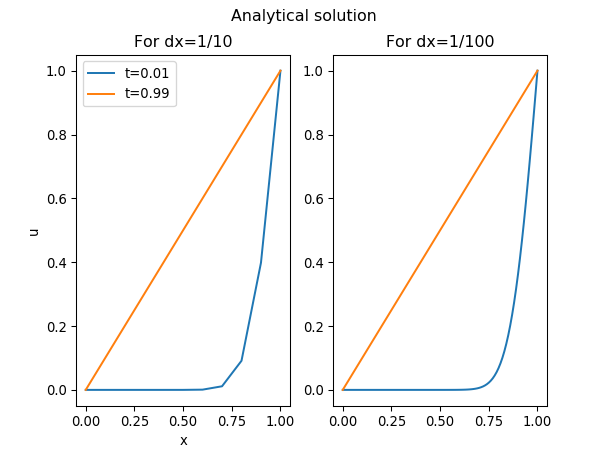
\includegraphics[width=120mm]{b.png}
	\caption{.}
	\label{fig:b}
\end{figure}

\begin{figure}[H]
	\centering
	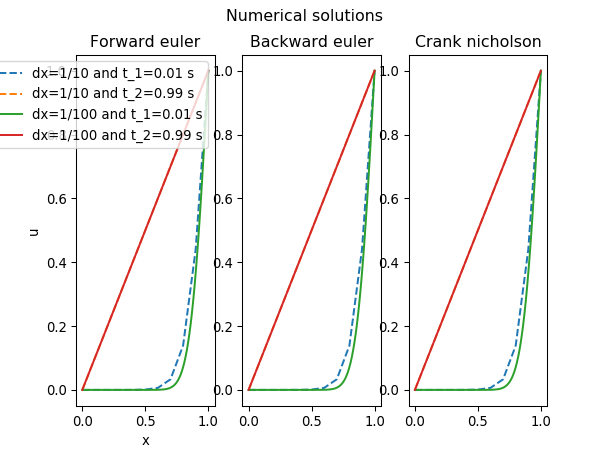
\includegraphics[width=120mm]{c.png}
	\caption{.}
	\label{fig:c}
\end{figure}

\subsection{Tables}


\begin{table}[H]
\begin{center}
\caption{Theoretical truncation errors.}
\begin{tabular}{  |c|c|c|c|c|c| } \hline
Scheme:&	Truncation error&Stability requirments \\ \hline
Crank Nicholson&$O(\Delta x^2) and O(\Delta t^2)$&Stable for all\\ \hline
Backward Euler&$O(\Delta x^2) and O(\Delta t^2)$&Stable for all\\ \hline
Froward Euler&$O(\Delta x^2) and O(\Delta t^2)$&$\Delta t \leq 1/2\Delta x^2$\\ \hline
\end{tabular}
\label{tab:a}
\end{center}
\end{table}

\section{Appendix}

The one dimensional diffusion equation has an analytical expression for the continuous problem. 

\begin{equation}
\nabla ^2 u(x,t)=\frac{\partial u(x,t)}{\partial t}
\label{eq:a1d}
\end{equation}

The initial condition is $u(x,0)=g(x)$, when $0<x<L$. We also have $u(0,t)=0$ and $u(L,t)=0$, when $t\leq0$. We use separation of variables when solving \ref{eq:a1d}:

\begin{equation}
u(x,t) = F(x)G(t)
\label{eq:sep}
\end{equation}

This gives us one function only depending on position x and one only depending on time t. We get the set of equations:

\begin{equation*}
\frac{\partial u}{\partial t} = F \frac{\partial G}{\partial t}
\end{equation*}

and

\begin{equation*}
\frac{\partial^2 u}{\partial x^2} = G \frac{\partial^2 F}{\partial x^2}
\end{equation*}

We can now use the relation given equation \ref{eq:heat_one}:

\begin{equation}
\begin{split}
&F\frac{\partial G}{\partial t} = G \frac{\partial ^2 F}{\partial x^2}\\
&\frac{1}{G}\frac{\partial G}{\partial t} = \frac{1}{F} \frac{\partial^2 F}{\partial x^2}
\end{split}
\end{equation}

We set the equations equal to a negative constant $-\lambda^2$. This gives us the solutions:

\begin{equation*}
\begin{split}
G &= Ae^{-\lambda^2 t}\\
F &= B\cos{(\lambda x)} + C\sin{(\lambda x)}
\end{split}
\end{equation*} 

We can now use equation \ref{eq:sep} to find the general solution u:

\begin{equation}
\begin{split}
u &= GF = Ae^{-\lambda^2 t} [B\cos{(\lambda x)} + C\sin{(\lambda x)}]\\
&=e^{-\lambda^2 t} [C_1\cos{(\lambda x)} + C_2\sin{(\lambda x)}]
\end{split}
\end{equation}

The boundary conditions gives us the solution:

\begin{equation}
u(x,t) = A_n\sin{(n\pi x/L)}e^{-n^2\pi^2t/L}
\end{equation}

We have infinitely many solutions to this equation, due to the n factor. We can use a superposition of these solutions since the diffusion equation is linear:

\begin{equation}
u(x,t) = \sum_{n=1}^{\infty}A_n\sin{(n\pi x/L)}e^{-n^2\pi^2t/L}
\label{eq:u_undfA}
\end{equation}

We decide the coefficient $A_n$ by using the initial condition:

\begin{equation}
u(x,0)=g(x)=\sum_{n=1}^{\infty}A_n\sin{(n\pi x/L)}
\end{equation}

Which gives us that:

\begin{equation*}
A_n=\frac{2}{L}\int_0^Lg(x)\sin{(n\pi x/L)} dx
\end{equation*}

We need to find the function g(x). We should obtain an equilibrium temperature when the time goes to infinity. This can be written as:

\begin{equation*}
\lim_{t \to \infty} u(x,t) = u_E(x)
\end{equation*}

Where $u_E(x)$ is the equilibrium temperature. We can look at how this function behaves given the boundary conditions:

\begin{equation*}
\frac{d^2 u_E}{dx^2}=0 \hspace{0.5cm} u_E(0)=0\hspace{0.5cm} u_E(L)=1
\end{equation*}

This gives us the general solution:

\begin{equation*}
u_E(x)=k_1x + k_2
\end{equation*}

Where $k_1$ and $k_2$ are constants. We get the function $u_E(x)=x/L$. Now we define a new function $v(x,t)=u(x,t)-u_E(x)$, where $u(x,t)$ is the solution to equation \ref{eq:u_undfA}, which we wish to solve for:

\begin{equation}
u(x,t)=v(x,t)+u_E(x)
\label{eq:vu}
\end{equation}

We need to know the boundary and initial conditions for $v(x,t)$:

\begin{equation*}
\begin{split}
&v(x,0)=u(x,0)-u_E(x)=0-x/L=-x/L\\
&v(0,t)=u(0,t)-u_E(0)=0-0=0\\
&v(L,t)=u(L,t)-u_E(L)=1-1=0
\end{split}
\end{equation*}
 
 We use the same method as earlier and find the solution for v(x,t):
 
 \begin{equation}
v(x,t) = \sum_{n=1}^{\infty}B_n\sin{(n\pi x/L)}e^{-n^2\pi^2t/L}
\end{equation}
 
Where the coefficient $B_n$ is given by:

\begin{equation}
B_n=\frac{2}{L}\int_0^Lg(x)\sin{(n\pi x/L)} dx
\end{equation}

Now we can use the fact that g(x)=v(x,0)=-x/L and equation \ref{eq:vu}:

\begin{equation}
u(x,t)=x/L+\sum_{n=1}^{\infty}\frac{2}{L}\int_0^L(-x/L)\sin{(n\pi x/L)} dx\sin{(n\pi x/L)}e^{-n^2\pi^2t/L}
\end{equation}

We solve the integral and find the final solution:

\begin{equation*}
\begin{split}
&\int_0^L(-x/L)\sin{(n\pi x/L)} dx=\frac{L(\pi n \cos{(\pi n)}-\sin{(\pi n)})}{\pi^2n^2}\\
&\Rightarrow u(x,t)=x/L+\sum_{n=1}^{\infty}\frac{2(\pi n \cos{(\pi n)}-\sin{(\pi n)})}{\pi^2n^2}\sin{(n\pi x/L)}e^{-n^2\pi^2t/L}
\end{split}
\end{equation*}

We now have a analytical expression for heat diffusion in one dimension \cite{94}\cite{96}. 


\begin{thebibliography}{9}
\bibitem{94}
	Jensen, M.H., 2015, Computational Physics Lecture Notes Fall 2015
\bibitem{95}
	Jensen, M.H., 2017, Computational Physics Lectures: Statistical physics and the Ising Model
\bibitem{96}
	Dawkins, Paul., 2018, Heat Equation With Non-Zero Temperature Boundaries
\bibitem{97}
	Despotovic, M, et al., 2016, Evaluation of empirical models for predicting monthly mean horizontal diffuse solar radiation
	
\end{thebibliography}

\end{document}